\documentclass[conference]{IEEEtran}
\IEEEoverridecommandlockouts
% The preceding line is only needed to identify funding in the first footnote. If that is unneeded, please comment it out.
\usepackage{cite}
\usepackage{tikz}
\usetikzlibrary{shapes.geometric, arrows, positioning}
\usepackage{amsmath,amssymb,amsfonts}
\usepackage{comment}
\usepackage{algorithmic}
\usepackage{graphicx}
\usepackage{textcomp}
\usepackage{float}
\usepackage{xcolor}
\def\BibTeX{{\rm B\kern-.05em{\sc i\kern-.025em b}\kern-.08em
    T\kern-.1667em\lower.7ex\hbox{E}\kern-.125emX}}
\begin{document}

\title{Combining Technical Indicators and Genetic Algorithms for Short-Term Machine Learning Prediction of Mini-Index Futures \\
%{\footnotesize \textsuperscript{*}Note: Sub-titles are not captured in Xplore and
%should not be used}
%\thanks{Identify applicable funding agency here. If none, delete this.}
}

\begin{comment}
\author{\IEEEauthorblockN{1\textsuperscript{st} Andrey V.S Souza}
\IEEEauthorblockA{\textit{Federal University of Rio Grande} \\
\textit{(FURG)}\\
Rio Grande, Brazil \\
0009-0006-4177-758X}
\and


\IEEEauthorblockN{2\textsuperscript{nd} Bruno L. Dalmazo}
\IEEEauthorblockA{\textit{Federal University of Rio Grande} \\
\textit{(FURG)}\\
Rio Grande, Brazil \\
0000-0002-6996-7602}
\and

\IEEEauthorblockN{3\textsuperscript{rd}Viviane L.D de Mattos}
\IEEEauthorblockA{\textit{Federal University of Rio Grande} \\
\textit{(FURG)}\\
Rio Grande, Brazil \\
0000-0002-3512-6290}
\and


\hspace*{0.8cm}
\IEEEauthorblockN{4\textsuperscript{th} Richard F. Pinto}
\IEEEauthorblockA{\textit{ \hspace*{0.8cm} Federal University of Rio Grande} \\ \hspace*{0.9cm}
\textit{(FURG)}\\ \hspace*{0.9cm}
Rio Grande, Brazil \\ \hspace*{0.9cm}
0009-0007-0176-3383}
\and

\IEEEauthorblockN{5\textsuperscript{th}Diego R. Bruno}
\IEEEauthorblockA{\textit{Universidade Estatual Paulista} \\
\textit{(UNESP)}\\
São Paulo, Brazil \\
0009-0008-1806-0278}
\and

\IEEEauthorblockN{6\textsuperscript{th} Eduardo N. Borges}
\IEEEauthorblockA{\textit{Federal University of Rio Grande} \\
\textit{(FURG)}\\
Rio Grande, Brazil \\
0000-0003-1595-7676}
\and

\hspace*{1cm}
\IEEEauthorblockN{7\textsuperscript{th} Giancarlo Lucca}
\IEEEauthorblockA{\textit{ \hspace*{1cm} Federal University of Pelotas} \\\hspace*{1.0cm}
\textit{(UFPel)}\\ \hspace*{1.0cm}
Pelotas, Brazil \\ \hspace*{1.0cm}
0000-0002-3776-0260}
\and

\hspace*{2cm}
\IEEEauthorblockN{8\textsuperscript{th} Fabian C. Cardoso}
\IEEEauthorblockA{\textit{ \hspace*{2cm} University of Rio Verde} \\
\hspace*{2cm}
\textit{(UniRV)}\\ \hspace*{2cm}
Rio Verde, Brazil \\ \hspace*{2cm}
0000-0002-2842-0387}
\and

\and
\hspace*{0.9cm}
\IEEEauthorblockN{9\textsuperscript{th} Rafael A. Berri}
\IEEEauthorblockA{\textit{ \hspace*{0.9cm} Federal University of Rio Grande} \\\hspace*{0.9cm}
\textit{(FURG)}\\\hspace*{0.9cm}
Rio Grande, Brazil \\\hspace*{0.9cm}
0000-0002-3812-4186}
}
%name of organization (of Aff.)
\end{comment}

\maketitle
\begin{abstract}
This article investigates short-term trend forecasting in the mini-index futures market using a hybrid framework that integrates technical analysis, feature selection, and evolutionary hyperparameter optimization. Five-minute intraday data obtained from the BovDBV2 database are used to construct a set of technical indicators that capture short-term price dynamics. To address the redundancy and noise commonly found in high-dimensional financial data, a feature selection method is applied to reduce the original feature space to a compact and informative subset. Genetic algorithms are then employed to optimize the hyperparameters of three supervised learning models: Random Forest, Support Vector Machine, and Multilayer Perceptron.

Experimental results indicate that genetic algorithm optimization consistently improves model performance when compared to a baseline Random Forest model without hyperparameter tuning, which achieved an accuracy of approximately 61.63\%. Within the proposed framework, the optimized Support Vector Machine and Multilayer Perceptron models reach test accuracies of 65.61\% and 65.85\%, respectively, while maintaining balanced $F1-scores$ across uptrend and downtrend classes. These results demonstrate the effectiveness of combining feature selection with evolutionary hyperparameter optimization for short-term financial time series forecasting in derivatives markets.
\end{abstract}

\begin{IEEEkeywords}
Neural Network, Machine Learning, Genetic Algorithm, Intraday Trading, Mini Index
\end{IEEEkeywords}



\section{Introduction}

The financial market is the arena for investing in various capital instruments traded to achieve economic returns and manage risk. One of the most sought-after assets by investors is futures contracts, noted for their high liquidity; they are widely used for both hedging against price fluctuations and speculative strategies. These contracts establish the purchase or sale of an underlying asset at a predetermined price, with settlement on a future date, making them particularly sensitive to market expectations and short-term dynamics \cite{jarrow1981forward}.

Data generated from trading on stock exchanges worldwide enables the development of assets with both short- and long-term horizons to identify return patterns that support investment strategies. However, many of these patterns tend to dissipate as the market exploits them, reinforcing the dynamic and uncertain nature of financial series.

In Brazil, the Brazilian Stock Exchange (B3\footnote{https://www.b3.com.br/}) stands out as the main regulated trading environment in the country. Among them, the Mini Index (WIN) futures contract, referenced to the Ibovespa, has high liquidity and is widely used in short-term strategies and intraday operations, making it a particularly relevant source of data for computational studies of financial time-series forecasting.

Early attempts to standardize patterns and identify trends used static, linear models, such as traditional time-series methods %\cite{box2015time}%.
As finance and computing converged (Stock Market Prediction) \cite{jiang2021applications}, more sophisticated models, such as machine learning (ML) algorithms, gained popularity for market forecasting. Recently, deep learning architectures such as Multilayer Perceptrons (MLPs) and recurrent neural networks have expanded these techniques, enabling the learning of complex patterns from historical data.

A key part of data-driven methods involves technical analysis using indicators such as moving averages and volatility, which capture market trends for machine learning \cite{nabipour2020predicting}. However, the high dimensionality and redundancy of raw indicators challenge model training, making feature selection vital to find the most useful ones. Model performance also relies on proper hyperparameter tuning, where meta-heuristic techniques like Genetic Algorithms (GA) \cite{chung2018genetic} effectively explore complex settings and avoid local optima, unlike gradient-based methods.

The objective of this article is to investigate how evolutionary optimization strategies scale with more expressive and sensitive learning models for intraday financial forecasting. While feature selection with a Random Forest (RF) baseline has proven effective, these methods do not always generalize to classifiers with greater representational power and risk of overfitting. Here, we extend prior research by jointly optimizing feature subsets and hyperparameters for Support Vector Machines (SVM) and Multilayer Perceptrons using a unified genetic framework, systematically evaluating robustness and generalization in financial time series forecasting.



The structure of this article is as follows: Section ~\ref{sec:relatedwork} presents related works. Section ~\ref{sec:Methodology} describes the methodology adopted in this study. Section ~\ref{sec:results} presents and discusses the experimental results. Finally, Section ~\ref{conlusion} presents the conclusions and directions for future research.


\section{Related Work}
\label{sec:relatedwork}
With the advancements in artificial intelligence and the widespread use of concepts such as \textit{machine learning} and \textit{deep learning} in the literature, various sectors—both academic and industrial—have sought to apply these techniques to their respective domains. One of these areas is the financial market \cite{heaton2017deep}, where the ability to predict future market values has attracted considerable attention.

In research by Ballings \cite{ballings2015evaluating}, various machine learning techniques were tested for stock market prediction using financial data from 5,767 European companies. Experimental results identified SVM as the most accurate model, followed by Random Forest, Kernel Factory, AdaBoost, and Logistic Regression. These findings highlight the adaptability of machine learning for financial forecasting and show that model performance depends strongly on input feature selection, hyperparameter tuning, and learning strategies.

In this scenario, the MLP has become a widely used deep learning architecture in financial forecasting, primarily because it can capture complex nonlinear relationships among economic variables. F. Ecer ~\cite{ecer2020training} proposed an optimized MLP architecture for financial time-series forecasting, evaluating various network topologies and activation functions.


Recent studies show technical analysis indicators are effective features for machine learning in stock prediction. Naik and Mohan 
\cite{naik2019optimal} used Boruta to select relevant indicators from 33 combinations, finding dimensionality reduction boosts short-term prediction accuracy. Their ANN model cut prediction error by 12\% on NSE data, highlighting the value of selecting informative features from high-dimensional sets.

Hyperparameter optimization is vital for neural network performance in finance. Ding et al. \cite{ding2011optimizing} introduced a hybrid GA-Back-Propagation (BP) approach to overcome BP networks' limitations, combining GA's global search with BP fine-tuning for better generalization on UCI datasets.

Unlike previous studies that treat feature selection and hyperparameter tuning separately, this work integrates both within a unified evolutionary framework and evaluates their effectiveness across distinct models for financial market time series prediction.

\section{Methology}
\label{sec:Methodology}

This section presents the methodology adopted in this study. Figure ~\ref{fig:overviewmethodology} presents an overview of the methodological flow adopted in this study. The diagram highlights each step of the process, illustrating the flow from data acquisition to model optimization and evaluation.

%coloquei a imagem para pegar duas colunas, não dá para ler da forma que estava.


\begin{figure}[H]
\centering
\resizebox{1\columnwidth}{!}{
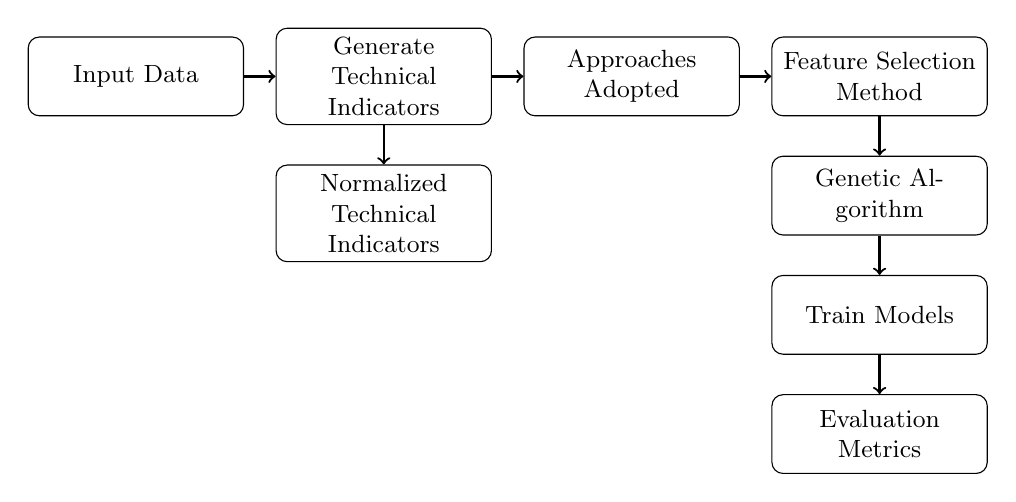
\begin{tikzpicture}[
    node distance=0.5cm and 0.4cm,
    every node/.style={
        draw,
        rounded corners,
        align=center,
        text width=2.5cm,
        minimum height=1.0cm,
        font=\small
    },
    arrow/.style={->, thick}
]

% --- Left side ---
\node (input) {Input Data};
\node (indicators) [right=of input] {Generate\\Technical Indicators};
\node (norm) [below=of indicators] {Normalized\\Technical Indicators};

% --- Middle ---
\node (approach) [right=of indicators] {Approaches\\Adopted};

% --- Right side (stacked, no overlap) ---
\node (fs) [right=of approach] {Feature Selection\\Method};
\node (ga) [below=of fs] {Genetic Algorithm};
\node (train) [below=of ga] {Train Models};
\node (eval) [below=of train] {Evaluation Metrics};

% --- Arrows ---
\draw[arrow] (input) -- (indicators);
\draw[arrow] (indicators) -- (approach);
\draw[arrow] (indicators) -- (norm);
\draw[arrow] (approach) -- (fs);
\draw[arrow] (fs) -- (ga);
\draw[arrow] (ga) -- (train);
\draw[arrow] (train) -- (eval);

\end{tikzpicture}
}
\caption{Overview of the proposed methodology.}
\label{fig:overviewmethodology}
\end{figure}

\begin{comment}
\begin{figure}[H]
\centering
\includegraphics[width=1\columnwidth]
{images/overview.png}
\caption{Methodology Process Overview.}
\label{fig:overviewmethodology}
\end{figure}
\end{comment}

\subsection{Input Data}
\label{sec:data}

The data used in this article were obtained from the BovDbV2 \cite{souza2024dataset} database, an extension of the original BovDb \cite{cardoso2022bovdb} that provides publicly available, pre-processed information from the B3 for research purposes, covering listed companies from 1995 to 2024. This new version also includes intraday records in 5-minute windows from January to June 2024, enabling a more detailed analysis of short-term market dynamics.

From this intraday data, a subset of futures contracts relevant to the objectives of this study was selected, with emphasis on the WIN, chosen for its high liquidity and suitability for short-term strategies. The contracts considered were WING24 and WINJ24 (Jan.–Feb. 2024), WINJ24 and WINM24 (Mar.–Apr. 2024), and WINM24 and WINQ24 (May–Jun. 2024), selected based on their high volumes and intense trading activity, totaling approximately 38 to 40 business days per period and more than 15,000 instances throughout the analyzed set.

The technical analysis indicators used in this study were computed from these intraday series and serve as the explanatory variables in the dataset. In addition, a binary market trend column was defined, with 0 indicating a downtrend and 1 indicating an uptrend. These labels were derived from a top and trough identification algorithm presented in previous work.


\subsection{Generation of Technical Analysis Indicators}
\label{sec:indicators}

Technical indicators were built from the intraday dataset to capture short-term price changes. Key metrics—Simple Moving Average (SMA), Exponential Moving Average (EMA), and Standard Deviation—were calculated using short time windows (3, 5, 7, and 9 periods) to enhance sensitivity to rapid market shifts, where significant moves can happen in minutes \cite{hunter1986exponentially}.

To capture changes in trend slope and momentum, attributes derived from the differences between calculated moving averages were also constructed. For example, the difference between the 7-period SMA and the 3-period SMA is defined in Eq. (1) as:

\begin{equation}
\text{SMA}_{7-3} = \text{SMA}_{7} - \text{SMA}_{3},
\end{equation}

A central preprocessing step consisted of normalizing the technical indicators \cite{singh2022feature}, as well as the opening and closing prices, in order to place all variables on a common numerical scale. For each 5-minute intraday window, a min–max–type scaling was applied, in which each feature was transformed according to Eq. (2):

\begin{equation}
\text{Feature}_{\text{norm}} = \frac{\text{Feature} - \text{Low}}{\text{High} - \text{Low}}.
\end{equation}

Where \textit{High} and \textit{Low} correspond to the maximum and minimum prices observed within the same 5-minute interval, and \textit{Feature} denotes any technical indicator or price-based variable being normalized. This transformation maps the features predominantly to the interval $[0,1]$, while preserving their relative positions within the intraday price range, thereby reducing the impact of heterogeneous attribute scales and facilitating the learning of machine learning models. This normalization procedure, combined with historical information on open, high, low, average, close, bid, ask, trade volume, and number of shares, results in a total of 66 constructed features.

\subsection{Feature Selection Method}
\label{sec:Feature Selection}
The predictive pipeline incorporates a structured feature selection stage based on technical analysis indicators. Following the approach proposed in \cite{souza2024dataset}, multiple selection strategies are evaluated to identify the most informative feature subsets, thereby enhancing model discrimination while reducing redundancy and noise inherent in high-dimensional financial data.

Based on the results presented, we evaluated several feature selection approaches using filters and wrappers. Among the methods evaluated, the \textit{Information Gain Method }\cite{lei2012feature} demonstrated superior performance in terms of model stability compared to all other methods tested, showing generalization and training efficiency when applied to the %our%
intraday dataset. This method identified a compact and informative subset, selecting 7 features from the original 66.

The selected features, ranked by their Information Gain scores, include the EMA-based differences $5\!-\!3$ and $7\!-\!3$, their normalized counterparts, the normalized 9-period SMA, the $9\!-\!3$ EMA difference, and the normalized 7-period EMA. 

This ranked subset was subsequently used as the optimized input space for training the models using a GA-based hyperparameter optimization procedure. Limiting the learning space to key indicators allowed the genetic algorithm's optimization to run more efficiently, finding parameters with better predictive capacity and less variance \cite{kumar2014feature}.

\subsection{Genetic Algorithm Parameters}
\label{sec:Genetic Algorithm Parameters}

Genetic Algorithms, grounded in the seminal works of Holland \cite{holland1984genetic} and Goldberg \cite{goldberg1989genetic}, constitute a class of evolutionary optimization methods particularly suitable for high-dimensional and multimodal search spaces. Their stochastic nature enables efficient global exploration, mitigating the risk of premature convergence that frequently affects gradient-based or exhaustive search strategies. These characteristics are especially relevant in financial time series modeling, where nonlinearity, structural regimes, and noise produce highly irregular loss surfaces.

A fixed configuration of GA parameters was used across all experiments to ensure methodological consistency and enable direct model-to-model comparison. The search proceeds through successive generations, with diversity enforced via uniform crossover and gene-wise mutation, and selective pressure maintained through tournament selection.

Evolutionary optimization was performed using a genetic algorithm with a population of 10 individuals evolved over 1,000 generations. Uniform crossover was applied with a probability of 0.80, and mutation was performed using a gene-wise adaptive strategy with a probability of 0.05 per individual and per gene. Parent selection was based on tournament selection with a tournament size of three individuals. Model fitness was evaluated using a parallel cross-validation strategy. The optimized hyperparameters from this configuration were then used to retrain the final predictive models.

\section{Results}
\label{sec:results}

This section presents the experimental results and discusses their implications for forecasting short-term movements in Brazilian Mini Index Futures Contracts. The analysis has two parts: the first describes the setup and evaluation protocol, and the second compares the models' predictive performance.

\subsection{Experimental Setup and Data Partitioning}

To ensure a fair and consistent comparison, all models evaluated in this study were trained and tested under identical experimental conditions. Each model used the reduced feature set from the feature selection stage, as described in Section~\ref{sec:Feature Selection}, consisting of seven technical indicators selected using the Information Gain criterion. In addition, all models used the same Genetic Algorithm configuration for hyperparameter optimization, as detailed in Section~\ref{sec:Genetic Algorithm Parameters}.

The dataset was split into training and test sets using a balanced, reproducible strategy to address class imbalance and temporal bias. From the intraday data, 1,500 ``uptrend'' and 1,500 ``downtrend'' instances were randomly sampled for the training set, creating a balanced 3,000-instance subset. A fixed seed ensured reproducibility. The remaining 12,057 instances were reserved for testing.

To obtain reliable estimates and reduce variance, all models used 5-fold cross-validation on the training set, splitting data into five folds, training on four, validating on one, and averaging accuracy. After optimization, models were retrained on all training data and tested on the unseen set.

All experiments were conducted in the same computational environment to ensure comparable execution times and performance metrics. The models were trained on a CPU-based system with 12 processing cores and 16 GB of RAM. In this configuration, the MLP required approximately 18 hours to complete optimization and training, while the SVM required approximately 3 hours and the RF approximately 2 hours. These differences reflect the computational complexity and search space associated with each genetically optimized algorithm.

The following subsection presents a comparative analysis of the predictive performance achieved by each model under this unified experimental framework.


\subsection{Performance of the Models}
\label{sec:performance_models}

This subsection presents and discusses the results obtained from training and evaluating the proposed models, with initial emphasis on the performance of the Random Forest model after hyperparameter optimization using the GA.

Table ~\ref{tab:rf_hyperparameters} shows the search space defined for each hyperparameter, as well as the optimal values found at the end of the evolutionary process. Each hyperparameter optimized by the GA plays a distinct role in controlling the complexity and generalization capacity of the RF model. The $\text{n\_estimators}$ parameter defines the number of decision trees in the ensemble; the $\text{max\_depth}$ parameter limits the maximum depth of each tree; the $\text{min\_samples\_split}$ parameter specifies the minimum number of samples required to split an internal node, acting as a regularization mechanism that prevents overly specific decision rules. Similarly, $\text{min\_samples\_leaf}$ determines the minimum number of samples required in a leaf node, resulting in smoother decision boundaries and increased robustness against noise. 

\begin{table}[ht]
\centering
\caption{Random Forest hyperparameters optimized by the Genetic Algorithm}
\label{tab:rf_hyperparameters}
\begin{tabular}{lcc}
\hline
\textbf{Hyperparameter} & \textbf{Search Space} & \textbf{Optimal Value} \\
\hline
$n\_estimators$      & $[50, 500]$          & 200   \\
$max\_depth$         & $[5, 50]$            & 15    \\
$min\_samples\_split$& $[2, 20]$            & 4     \\
$min\_samples\_leaf$ & $[1, 20]$            & 1     \\
\hline
\end{tabular}
\end{table}

Figure ~\ref{fig:ga_fitness_rf} shows the fitness evolution, measured as average accuracy from 5-fold cross-validation, across the GA generations for the Random Forest. It quickly converges initially and then stabilizes, indicating efficient hyperparameter exploration.

\begin{figure}[ht]
    \centering
    \includegraphics[width=1.0\linewidth]{images/garandomforestcopy.png}
    \caption{Evolution of the fitness function during the Genetic Algorithm optimization of the Random Forest model, where the x-axis denotes the generation number and the y-axis represents the average cross-validation accuracy.
}
    \label{fig:ga_fitness_rf}
\end{figure}


The best individual found by the Hall of Fame (HOF) showed an average cross-validation accuracy of $0.7739$.

In the test set, the model showed a final accuracy of 0.6331. RF analysis indicates a relatively balanced performance between the uptrend and downtrend classes, with comparable levels of recall and accuracy in both categories. Despite this balance, a non-negligible number of misclassifications occur in both directions. The resulting F1 values were 0.6169 for the downtrend class and 0.6479 for the uptrend class, reflecting moderate but consistent predictive performance.

The SVM classifier, optimized using a Genetic Algorithm, was configured with a Radial Basis Function (RBF) Kernel, particularly suitable for capturing nonlinear decision boundaries in high-dimensional feature spaces.

Figure~\ref{fig:ga_fitness_svm} shows the fitness function's evolution during the genetic algorithm's optimization of the SVM model. It improves quickly at first, then stabilizes, signifying convergence to a robust hyperparameter configuration.

\begin{figure}[ht]
    \centering
    \includegraphics[width=1.0\linewidth]{images/gasvmcopy.png}
    \caption{Evolution of the fitness function during the Genetic Algorithm optimization of the SVM model (RBF kernel), where the x-axis denotes the generation number and the y-axis represents the average cross-validation accuracy.}
    \label{fig:ga_fitness_svm}
\end{figure}

The best individual preserved by the HOF achieved a mean cross-validation accuracy of 0.6517, reflecting stable performance across folds and indicating adequate generalization during training.

\begin{table}[ht]
\centering
\caption{SVM hyperparameters and search space optimized by the Genetic Algorithm}
\label{tab:svm_hyperparameters}
\begin{tabular}{lcc}
\hline
\textbf{Hyperparameter} & \textbf{Search Space} & \textbf{Optimal Value} \\
\hline
$C$      & $\log_{10}(C) \in [-3, 3]$      & $9.75 \times 10^{2}$ \\
$\gamma$ & $\log_{10}(\gamma) \in [-5, 1]$ & $1.28 \times 10^{-5}$ \\
Kernel   & Fixed & RBF \\
\hline
\end{tabular}
\end{table}
Table \ref{tab:svm_hyperparameters} illustrates that the $C$ and $gamma$ hyperparameters shape the SVM's behavior; $C$ balances margin maximization and error minimization, with higher values favoring correct classification and complexity. $gamma$ determines the local influence radius, with smaller values smoothing boundaries and larger ones fitting localized patterns. Their combination affects the SVM's flexibility and generalization. On a test set of 12,057 unseen instances, the model achieved 0.6561 accuracy, outperforming the Random Forest. Like the Random Forest, the SVM achieved balanced performance across trend classes, with higher effectiveness for uptrend detection, resulting in F1-scores of 0.6308 and 0.6781 for downtrend and uptrend.

Following our approach, the Multilayer Perceptron classifier was optimized using a GA. The MLP represents a nonlinear parametric model capable of approximating complex decision boundaries through layered compositions of affine transformations and nonlinear activation functions, making it particularly suitable for financial time series classification problems.

The Genetic Algorithm was employed to optimize the architectural and training hyperparameters of the MLP, including the number of neurons in the hidden layer, the learning rate, the L2 regularization coefficient, the dropout rate, the batch size, the activation function, and the optimizer.


\begin{figure}[ht]
    \centering
    \includegraphics[width=1\linewidth]{images/gamlpcopy.png}
    \caption{Evolution of the fitness function during the Genetic Algorithm optimization of the MLP model, where the x-axis denotes the generation number and the y-axis represents the average cross-validation accuracy.}
    \label{fig:ga_fitness_mlp}
\end{figure}

Figure ~\ref{fig:ga_fitness_mlp} shows the fitness evolution over 1,000 generations of the GA. The best individual's curve improves gradually and stabilizes, indicating convergence to a local optimum. The average fitness varies more, reflecting the exploration and diversity of solutions.

The best individual identified by the HOF achieved a mean cross-validation accuracy of approximately $0.6540$, with observed fitness values ranging from $0.6499$ to $0.6540$ across generations. The optimal hyperparameter configuration obtained for the MLP model is summarized in Table~\ref{tab:mlp_hyperparameters}.

\begin{table}[ht]
\centering
\caption{MLP hyperparameters optimized by the Genetic Algorithm}
\label{tab:mlp_hyperparameters}
\begin{tabular}{lcc}
\hline
\textbf{Hyperparameter} & \textbf{Search Space} & \textbf{Optimal Value} \\
\hline
Hidden neurons        & $[5, 500]$            & 44 \\
Learning rate         & $[10^{-8}, 10^{-2}]$  & $4.70 \times 10^{-3}$ \\
$L_2$ regularization  & $[10^{-8}, 10^{-2}]$  & $4.48 \times 10^{-6}$ \\
Dropout rate          & $[0.00, 0.10]$        & 0.07 \\
Batch size            & $\{16, \dots, 128\}$  & 80 \\
Activation function   & Fixed                 & Tanh \\
Optimizer             & Fixed                 & RMSprop \\
\hline
\end{tabular}
\end{table}

The number of neurons in the hidden layer affects the MLP's capacity. The Genetic Algorithm selected a moderate size to balance expressiveness and overfitting. An optimized logarithmic learning rate ensures efficient, stable convergence. Small $L_2$ regularization penalizes large weights, producing smoother solutions. Dropout deactivates neurons during training, improving generalization by reducing co-adaptation.

The final evaluation across the test suite resulted in an overall accuracy of 0.6585, comparable to the SVM model and superior to the Random Forest model under identical experimental conditions, for the model using the Hyperbolic Tagent Activation Function and RMSprop optimizer.

According to the ranking report, MLP achieved an F1 score of 0.6397 for the downtrend class and 0.6753 for the uptrend class. These results indicate slightly higher sensitivity to upward market movements, which is particularly relevant in financial forecasting contexts, where accurate identification of positive trends can yield greater practical utility.

To evaluate the sensitivity of the Multilayer Perceptron to the optimization strategy, a second model test experiment was conducted using the same search space configuration shown in the previous test, as per Table \ref{tab:mlp_hyperparameters}, with the only modification being the optimization algorithm employed during training, which was Adam.

The best individual found by the GA in this configuration specified a hidden layer with 89 neurons, a learning rate of \(1.94 \times 10^{-3}\), an \(L_{2}\) regularization coefficient of approximately \(8.71 \times 10^{-8}\), a dropout rate of 0.01 and a batch size of 112, while keeping the hyperbolic tangent activation function as the nonlinear transformation in the hidden layer.

Table~\ref{tab:mlp_optimizer_comparison} compares two MLP models optimized with RMSprop and Adam, focusing on min/max GA fitness, final test accuracy, and metrics like AUC-ROC and AUC-PR.

\begin{table}[H]
\centering
\caption{Comparison of MLP performance using different optimizers optimized by the Genetic Algorithm}
\label{tab:mlp_optimizer_comparison}
\begin{tabular}{lcc}
\hline
\textbf{Metric} & \textbf{MLP + RMSprop} & \textbf{MLP + Adam} \\
\hline
GA Fitness (min) & 0.6499 & 0.6471 \\
GA Fitness (max) & 0.6540 & 0.6514 \\
Test Accuracy   & 0.6585 & 0.6544 \\
Precision       & 0.6755 & 0.6783 \\
Recall          & 0.6789 & 0.6623 \\
F1-score        & 0.6772 & 0.6702 \\
AUC-ROC         & 0.7032 & 0.7023 \\
AUC-PR          & 0.7029 & 0.7022 \\
\hline
\end{tabular}
\end{table}


Table~\ref{tab:mlp_optimizer_comparison} shows both optimizers have similar probabilistic performance, with nearly identical AUC-ROC and AUC-PR values. The RMSprop-based MLP has slightly higher cross-validation fitness and test accuracy, while Adam yields a marginally higher F1-score, indicating the optimizer mainly influences the precision-recall trade-off rather than causing significant performance differences in the GA search space.

\begin{figure}[H]
    \centering
    \includegraphics[width=1\linewidth]{images/all_models.png}
    \caption{Comparison of training and test accuracy of all models.}
    \label{fig:models_cv_test_comparison}
\end{figure}


To place these results in a broader context, Figure~\ref{fig:models_cv_test_comparison} summarizes the cross-validation and test accuracies obtained by all models evaluated in this study, namely Random Forest, SVM, MLP with RMSprop and MLP with Adam. The image shows that, despite the Random Forest achieving the highest cross-validation accuracy, its performance deteriorates more sharply on the test set, whereas SVM and both MLP variants exhibit more consistent behavior between validation and test, with MLP (RMSprop) and SVM obtaining the best overall test accuracies among the compared approaches.

\section{Conclusion}
\label{conlusion}

This work extends the findings of \cite{souza2025predictive}, which investigated feature selection strategies for machine learning models applied to the Brazilian derivatives market. In that study, technical indicators extracted from intraday Mini-Index futures data were used to construct a reduced feature space, improving generalization and reducing computational cost. However, the Random Forest classifier, trained without hyperparameter optimization, achieved a test accuracy of approximately 61.63\%, indicating that feature selection alone is insufficient to fully address the complexity of intraday financial dynamics.

Building upon this foundation, this study advances the analysis by using a Genetic Algorithm–based hyperparameter optimization and evaluating more expressive learning models. Consistent performance gains across classifiers suggest a highly nonconvex optimization landscape, favoring evolutionary strategies over manual or heuristic tuning. While Random Forest led in cross-validation accuracy, Support Vector Machines and Multilayer Perceptrons better balanced cross-validation and out-of-sample performance.

This behavior shows that margin-based learning and deep networks perform better at capturing the unpredictable nature of high-frequency financial data. In particular, the Multilayer Perceptron trained with RMSprop reached the highest test accuracy, about 65.85\%.

Overall, these findings reinforce the effectiveness of combining feature selection with evolutionary hyperparameter optimization, especially when coupled with nonlinear models. From a methodological perspective, this study supports the use of hybrid evolutionary–machine learning frameworks as a robust approach to short-term forecasting in derivatives markets. It also provides insights that can be generalized to other noise-dominated, nonstationary prediction tasks.




\section*{Acknowledgment}
This information has been omitted to allow for blind
review.
\begin{comment}
The authors would like to thank FAPERGS (24/2551-
0001396-2, 23/2551-0000773-8), CNPq (305805/2021-5), FAPERGS/CNPq
(23/ 2551-0000126-8), and Fabian Cardoso would like to thank to Fesurv-University of Rio Verde.
\end{comment}


%\section*{References}

\bibliographystyle{IEEEtran}
\bibliography{cite}

\end{document}
